\clearpage
\chapter{Modelo de Datos}

\section{Justificación}
\paragraph{Para la aplicación final, se hará uso de un modelo de base de datos orientado a grafos. También se contará con un esquema no relacional, es decir, se carece de una normalización definida, perteneciente a la categoria NoSQL.}
\paragraph{ Las características de una base de datos NoSQL son las siguientes: }

\begin{itemize}
  \item Modelo de datos flexible.
  \item Buen rendimiento en clusters. 
  \item Sin esquemas.
\end{itemize}

\paragraph{Este tipo de bases resultan útiles debido a que se se pretende procesar grandes volúmenes de información.}

\paragraph{Las tecnologías para grandes volumenes de información son relativamente nuevas; estas surgieron debido a la necesidad que tenían empresas grandes como Google y Amazon.} 

\paragraph{La información fue convertida de un modelo relacional a un modelo basado en documentos, jerárquico o basado en columnas usando proceso de denormalización, ésto con la finalidad de dar un orden a la información considerando simplemente consultas de cierto tipo evitando así operaciones típicas del álgebra relacional cómo el Producto Cartesiano, que implicaba el uso de grandes recursos.}

\paragraph{Las tecnologías de tipo NoSQL se orientan a consultas y no a transacción. Lo que brinda un fácil acceso a la información, una estructura de los datos orientada a su posterior análisis, respuestas en tiempo real y una gran capacidad de escalar y replicar.}

\paragraph{Empresas cómo Foursquare, Google, Amazon, Uber o Twitter, han optado por complementar la información que persisten de forma relacional con modelos orientados a documentos usando tecnologías como Hbase, MongoDB, BigTable, DynamoDB, por citar algunos ejemplos.}

\section{Descripción}
\paragraph{Considerando la problematica y solución que plantea el equipo de Ambienta2MX, se ha optado por orientar el sistema a consultas usando documentos como modelo de datos base. }

\paragraph{La información que será guardada y posteriormente consultada por otros módulos del sistema seguirá un esquema propuesto por el equipo de trabajo, éste recopila la estructura de evaluaciones básicas generadas en practicamente cualquier tipo de articulos, peliculas, platillos, libros, entre otros como podemos ver en el siguiente diagrama de grafos.}

\newpage
    \begin{landscape}
      \begin{figure}[h!]
      \centering
      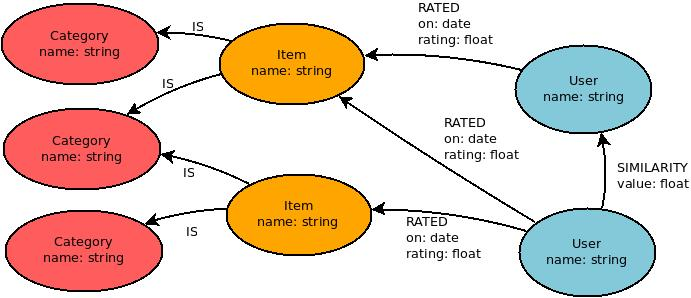
\includegraphics[width=22.5cm,height=12cm]{./images/Diagrama_general_datos.jpg}
      \caption{Modelo general necesario para el manejo de la información}
    \end{figure}
    \end{landscape}
  \newpage

\paragraph{Los documentos serán almacenados considerando los datos definidos en la especificación JSON Data Interchange Format (en su versión 2013). \cite{16}}

\paragraph{Se ha considerado el uso de el formato antes mencionado debido a su facilidad de lectura e integración con otro tipo de plataformas y lenguajes de programación, actualmente es el formato que rige el manejo de API de tipo REST.}

\paragraph{Dentro del modelo de la aplicación final se toma en cuenta el modelo general mínimo necesario para trabajar la información añadiendo información relevante. Considerando al final los siguientes documentos.}

\begin{itemize}
  \item Platillos
  \item Usuarios
  \item Restaurantes
  \item Categorias 
\end{itemize}

\paragraph{Para la información de los restaurantes, el modelo  permitirá almacenar la fuente de información externa en caso de ser utilizada para obtener datos adicionales a los que se poseen en la base de datos de acuerdo a registros como los contenidos por Foursquare en su API para la búsqueda de restaurantes.}

\paragraph{Las relaciones posibles entre los elementos Usuario, Restaurante, Platillo y sus posibles Categorias son visualizados en el siguiente diagrama.}

\newpage
    \begin{landscape}
      \begin{figure}[h!]
      \centering
      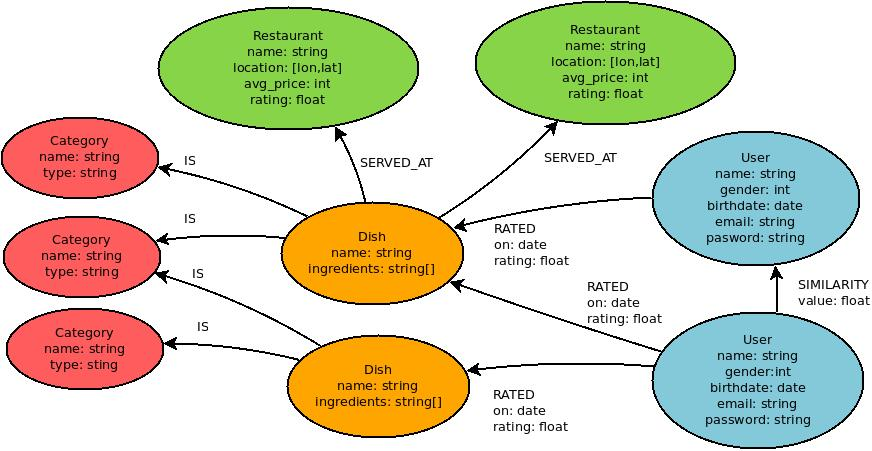
\includegraphics[width=22.5cm,height=12cm]{./images/Modelo_datos.jpg}
      \caption{Modelo propuesto para el caso de estudio}
    \end{figure}
    \end{landscape}
  \newpage

\newpage
\subsection{Modelo de datos}
  \lstinputlisting[language=Javascript]{../Resources/Model.js} 

\subsection{Categorias propuestas}
  \lstinputlisting[language=Javascript]{../Resources/Categories.js} 

